% Use the following line for draft mode (double spaced, single column)
\documentclass[preprint,pre,floats,aps,amsmath,amssymb]{revtex4}

% Use the following line for journal mode (single spaced, double column)
%\documentclass[twocolumn,pre,floats,aps,amsmath,amssymb]{revtex4}

\usepackage[]{graphicx}
\usepackage{subcaption}
\captionsetup{compatibility=false}
\usepackage{wrapfig} %for wrapping text around images
\usepackage{bm} %bold fonts, e.g. vectors
\usepackage{multirow} %multirow in tables
\usepackage{braket} %bra-ket notation
\usepackage{afterpage} %when you need clearpage, but don't want an empty page
%\renewcommand{\baselinestretch}{1} %for single-spaced

\graphicspath{{pics/}}


\begin{document}

\title{HgCr$_2$Se$_4$ as a Weyl semimetal}
\author{M\'{a}t\'{e} Hartstein}
\email{mate.hartstein@chch.ox.ac.uk}
\affiliation{Christ\:Church, University\:of\:Oxford}
\date{\today}

\clearpage\maketitle
\thispagestyle{empty}

%%%%%%%%%%%%%%%%%%%%%%%%%%%%%%%%%%%%%%%%%%%%%%%%%%%%%%%%%%%
%%%%%%%%%%%%%%%%%%%%%%%%%%%%%%%%%%%%%%%%%%%%%%%%%%%%%%%%%%%

\section{Introduction}
\label{sec:intro}

Topological insulators have become a widely pursued subject in condensed matter physics. A recently proposed related phase is the Weyl semimetal phase (Wan et al. (2011) \cite{wan}), which is also gaining popularity, with important experimental results yet to come.
 
This phase is identified by a band structure where two bands accidentally touch at isolated points in the Brillouin zone, which are reminiscent of massless Dirac fermions (or so-called Weyl fermions). This is subject to the condition that bands are non-degenerate, which also means that at least one of time reversal or inversion symmetry is broken. In contrast 3D topological insulators require unbroken TRS.
It has also been predicted by Wan et al. \cite{wan}, that bound states on certain surfaces form ``{Fermi arcs}", a really new and striking phenomenon, that has not been discussed outside of superconductivity. These proposals provide plenty of motivation for future experiments.
 
HgCr$_2$Se$_4$ is one of the few real materials that has been proposed to exhibit WSM related phases. This sparked a very recent interest in the material, leading to papers exploring the implications via theoretical predictions and various calculations. This report is to summarize older findings about its more fundamental properties, and recent results that could guide experimental work on HgCr$_2$Se$_4$.


%%%%%%%%%%%%%%%%%%%%%%%%%%%%%%%%%%%%%%%%%%%%%%%%%%%%%%%%%%%
%%%%%%%%%%%%%%%%%%%%%%%%%%%%%%%%%%%%%%%%%%%%%%%%%%%%%%%%%%%

\section{Structure}

HgCr$_2$Se$_4$ belongs to the spinel group. Consequently it has spinel crystal structure (shown in Fig.~\ref{spinel}, space group Fd$\bar3$m). This subclass of compounds is characterized by having the octahedral sites around the central atom (Hg in this case) occupied by magnetic ions (Cr$^{3+}$) and the tetrahedral sites occupied by a nonmagnetic ions (Se$^{2-}$). A more intuitive approach is to say, that there is a Hg atom at each fcc site, surrounded by tetrahedrons formed by four nonmagnetic ions, Se (these tetrahedrons can be seen in the schematic figure). Then each Cr is located in such a way, that they are octahedrally coordinated by the 6 nearest Se atoms. Table 1. lists, among other properties, the lattice constant, which was found to be 10.753 \AA by Baltzer et al. \cite{baltzer}. This is one of the earliest papers on HgCr$_2$Se$_4$, and was first to establish some of the more fundamental properties of the material. 


\begin{figure}[h]
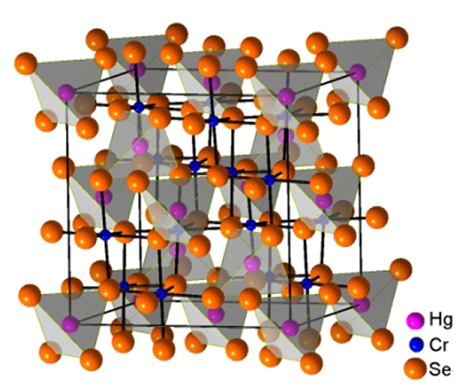
\includegraphics[height=0.57\linewidth]{spinel2.png}
\centering\captionof{figure}{The spinel crystal structure of HgCr$_2$Se$_4$ with Hg atoms in zinc-blende structure, each of them surrounded by Se tetrahedrons \cite{wang}. \label{spinel}}
\end{figure}

\begin{table}[h]
\centerline{\begin{tabular}{r|c|c|c|c|c|c|c}
  \hline \hline
   & \parbox{1.75cm}{Lattice parameter (\AA)} & \parbox{2.1cm}{Band gap, $\Delta$E$_g$ at 300 K (eV)} & \parbox{2.1cm}{ Resistivity, $\rho$, at 300 K ($\Omega\cdot$cm)} & \parbox{2.5cm}{Mobility, $\rho$, at 300 K (cm$^2\cdot$V$^{-1}\cdot$s$^{-1}$)} & \parbox{2.35cm}{\vspace{0.1cm} Magnetic moment at 4.2 K  ($\mu_B$/molecule)} & \parbox{1.8cm}{Curie temp., $T_c$ (K )}& \parbox{1.8cm}{Curie-Weiss, $\theta$ (K)}\\
  \hline
  HgCr$_2$Se$_4$ & 10.753 & 0.80 & 0.7 & 30 & 5.64 & 106 & 200 \\
  \hline \hline
\end{tabular}}
\caption{Basic properties of HgCr$_2$Se$_4$ \cite{baltzer}\cite{lehmann}.} 
\end{table}
%& \parbox{1.8cm}{Curie constant, $C_M$} & 3.79

%%%%%%%%%%%%%%%%%%%%%%%%%%%%%%%%%%%%%%%%%%%%%%%%%%%%%%%%%%%
%%%%%%%%%%%%%%%%%%%%%%%%%%%%%%%%%%%%%%%%%%%%%%%%%%%%%%%%%%%

\section{Magnetic properties}

HgCr$_2$Se$_4$ can be characterized as a ferromagnet, with a Curie temperature of 106 K \cite{baltzer}. The magnetism in this material originates from the three 3d electrons of the Cr$^{3+}$ ions \cite{selmi}, with its magnetic moment per molecule approaching 6 $\mu_B$, the value for two bare Cr$^{3+}$ ions, as we decrease the temperature (see Fig.~\ref{temp}).

Magnetization curves explored by Baltzer et al. \cite{baltzer} show ``quick" saturation with field, which suggests very low magnetic anisotropy. This low anisotropy would be consistent with the vanishing orbital moment of Cr$^{3+}$\cite{baltzer}.

\noindent\begin{minipage}{0.46\linewidth}
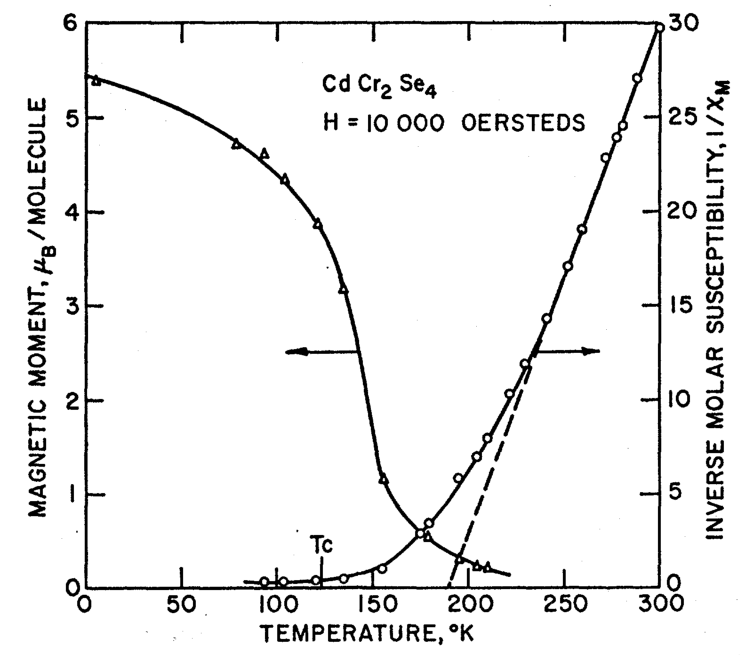
\includegraphics[width=1\linewidth]{momvstemp.png}
\centering\captionof{figure}{Magnetic moment and 1/$\chi$ as a function of temperature for CdCr$_2$Se$_4$. Similar behavior is expected for HgCr$_2$Se$_4$ \cite{baltzer}.\label{temp}}
\end{minipage}%
~ ~
\begin{minipage}{.55\linewidth}
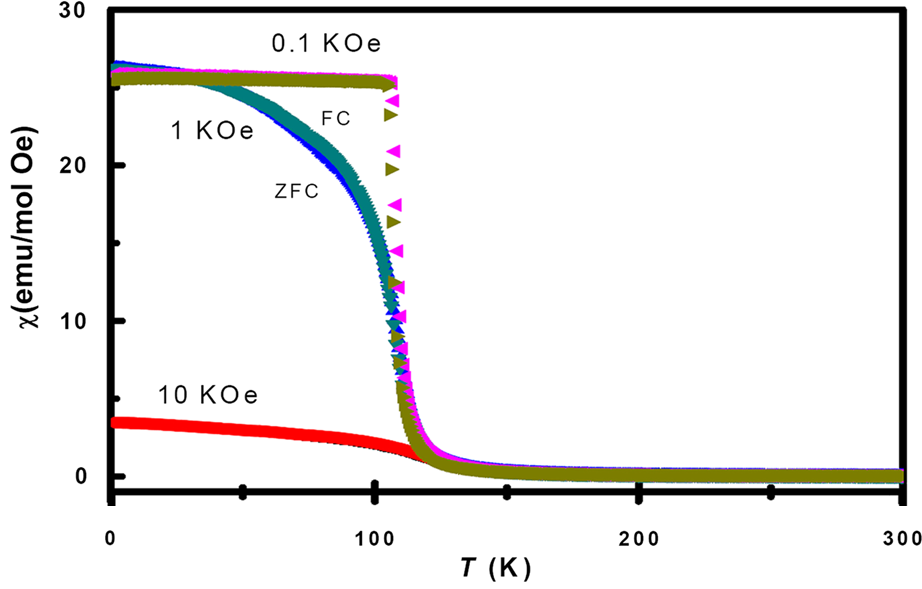
\includegraphics[width=1.05\linewidth]{suscvstemp.png}
\centering\captionof{figure}{Temperature dependence of the magnetic susceptibility for HgCr$_2$Se$_4$, clearly showing the phase transition \cite{wang}. \label{susc}}
%%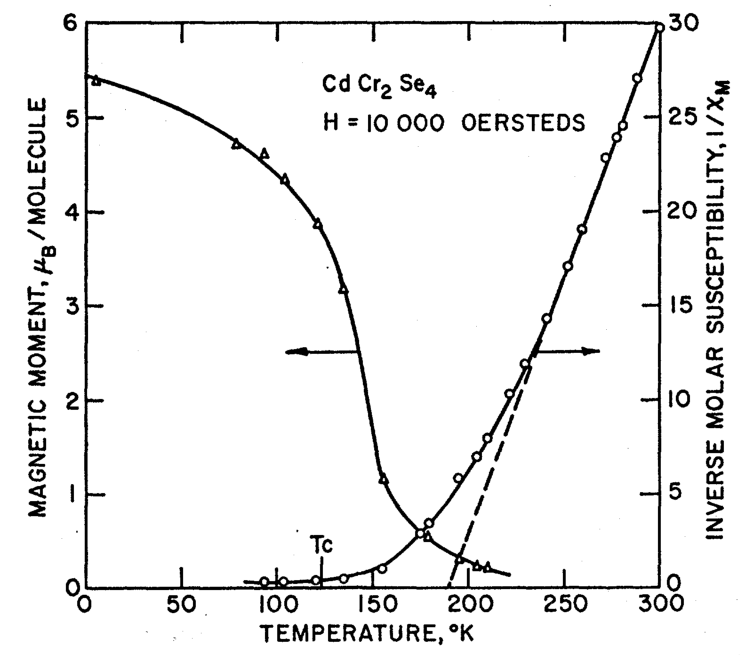
\includegraphics[height=0.95\linewidth]{momvstemp.png}
%\centering\captionof{figure}{Magnetic moment and inverse susceptibility as a function of temperature for CdCrgSe4 in an applied 6eld of 10000 Oe. HgCr$_2$Se$_4$ should have a similar behavior \cite{baltzer}.\label{field}}
\end{minipage}
\\

Two further findings need mentioning in this section. Firstly, the magnetoresistance of the material has been extensively explored, which lead to the relatively recent observation of colossal magnetoresistance in a layered structure of different conduction type HgCr$_2$Se$_4$ \cite{solin1}\cite{solin2}. Secondly, even though the antiferromagnetic (AFM) interaction is considered to be weak in the material, Wang et al. (2012) \cite{wang}, an extensive paper on the specific heat of the material, found that the competition between AFM and FM interactions becomes significant below low temperatures ($T < 3$ K) and magnetic fields (see Fig.~\ref{dheat}).

%%%%%%%%%%%%%%%%%%%%%%%%%%%%%%%%%%%%%%%%%%%%%%%%%%%%%%%%%%%
%%%%%%%%%%%%%%%%%%%%%%%%%%%%%%%%%%%%%%%%%%%%%%%%%%%%%%%%%%%


\section{Transport properties: resistivity and hall effect}

HgCr2Se4 is an electrical insulator in addition to being a ferromagnet, which is a rarity. It has the smallest band gap among the chromium spinels.

It is hard to pin down the transport characteristics as different measurements of the conductivity report different curves (see Fig.~\ref{mobility} \& Fig.~\ref{resi}) \cite{selmi}\cite{solin2}\cite{goldstein}, but it can generally be said that the material exhibits insulating/semiconducting character in the paramagnetic state, but metallic in the low temperature FM phase \cite{xu}.  Annealing has a strong influence on this, as it allows us to change a p-type sample (semiconducting) to n-type (insulating). 

For further insight, let us look at  Fig.~\ref{resi} by  Solin et al. (2007) \cite{solin2}. All crystals exhibit a sharp maximum of $\sigma$ near the Curie temperature $T_c \approx$ 106 K and a semiconductor-metal transition with decreasing temperature. Samples 2 and 3 reveal the semiconductor-metal-type transition at temperatures 25-30 K below T$_c$= 106 K. This crossover is also accompanied by inversion of conduction type from hole to electronic (see inset in Fig.\ref{resi}).

Selmi et al. (1985) \cite{selmi} lists similar results; their study  defined class I samples as those which fulfill the condition $n$(4.2 K) \textgreater~$2\cdot10^{-3}$ cm$^{18}$, so n-type. The main feature of such samples is that $n$ is roughly independent of $T$ below 200 K. To the contrary, for class II samples (n $\le$ $2\cdot10^{-3}$ cm$^{18}$), a sharp drop of $n$ at $T$ $\sim$ 120 K is observed, responsible for the peak of resistivity near T$_c$. In particular, the Hall mobility $\mu$ decreases monotonically near T$_c$ on all samples. It is established\cite{veselago} that the transport properties of undoped HgCr2Se4 single crystals are determined more by deviations from stoichiometry in Hg and Se content than by the presence of some uncontrollable impurity.
 
To continue the list of unusual properties of the material, we bring the attention to Xu et al.'s (2011) \cite{xu} seminal paper on the band structure calculation of HgCr2Se4, which is also proposing that quantized anomalous Hall effect (Hall effect without an applied field) can be achieved in its quantum-well structure, with the quantized conductivity to increase in steps with sample thickness (in jumps of $2\cdot e^2 / h$). Since the paper this has been referred to as one of the expected properties of a real Weyl semimetal. \cite{ashby}

The list of unconventional properties expected from Weyl semimetals is an extensive one, and includes one more prediction about the transport properties of such a material: DC-conductivity at low temperatures. There has been one paper (Toda (1970) \cite{toda}) along the lines of this property, which reported a DC voltage produced in the sample a decrease at ferromagnetic resonance at 77 K. It attributed this result to s-d exchange interactions. It also reported spontaneous Hall effect at 77 K. 



\noindent\begin{minipage}{0.49\linewidth}
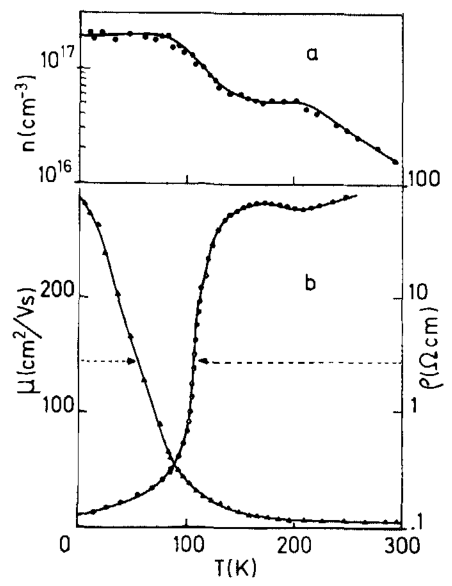
\includegraphics[height=1\linewidth]{mobvstemp.png}
\centering\captionof{figure}{Electron concentration, $n$ (a), mobility, $\mu$ , and resistivity, $\rho$ (b), vs.
temperature for the sample with smaller $n$ \cite{selmi}.\\ \\ \\ \\  \\ \\  \label{mobility}}
\end{minipage}%
~ ~
\begin{minipage}{.49\linewidth}
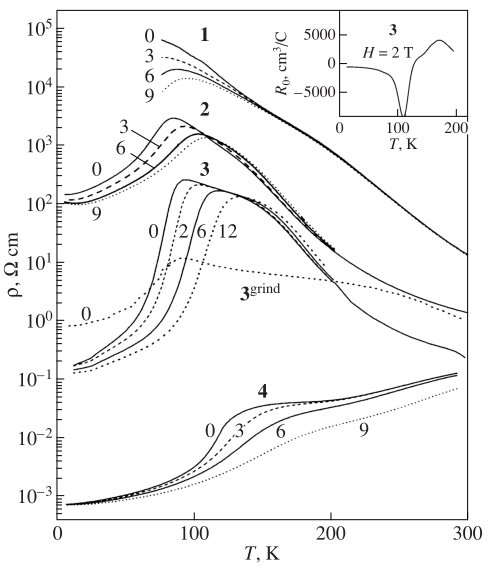
\includegraphics[height=1\linewidth]{resvstemp.png}
\centering\captionof{figure}{Temperature dependences of the electrical resistivity of single crystals as-grown (samples 1-3, which are p-type, n-type, n-type respectively) and annealed in mercury vapor (sample 4). The numbers adjoining the curves are magnetic fields in teslas. The inset shows the temperature dependence of the Hall constant for sample 3 measured at H = 2 T. \cite{solin2}.\label{resi}}
\end{minipage}

%%%%%%%%%%%%%%%%%%%%%%%%%%%%%%%%%%%%%%%%%%%%%%%%%%%%%%%%%%%
%%%%%%%%%%%%%%%%%%%%%%%%%%%%%%%%%%%%%%%%%%%%%%%%%%%%%%%%%%%

\section{Band structure}

As with most topological insulator candidates, there is a clear chronological gap in the distribution of papers on HgCr$_2$Se$_4$, with fundamental properties explored in the 60s and 70s, and theoretical calculations and simulations which are very recent, and can be tracked back to the seminal paper first proposing it as a candidate. Band structure papers are no different. 

Older papers found the band gap to be $\Delta$E$_g$= 0.80 eV at 300 K, and narrowing to 0.28 eV as one enters the ferromagnetic temperature domain \cite{lehmann}.

\noindent\begin{minipage}{0.5\linewidth}
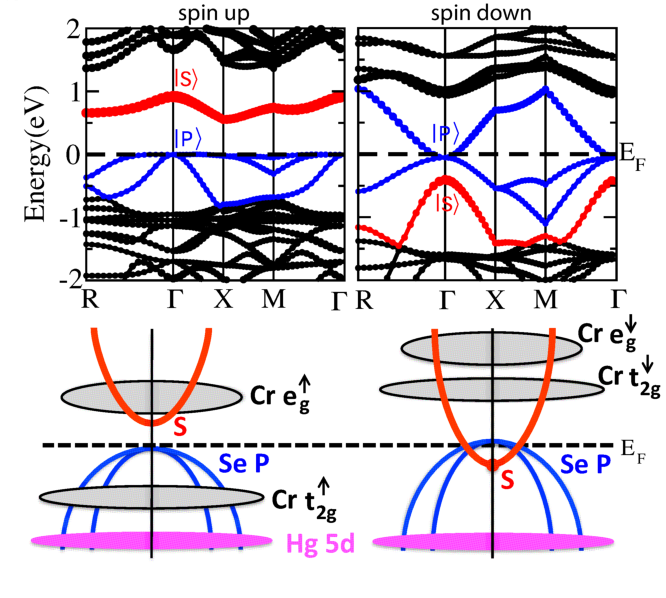
\includegraphics[width=1.07\linewidth]{bands0.png}
\centering\captionof{figure}{The upper pictures show the band structures without SOC (showing the up and down spin parts separately), while the lower pictures are the schematic understanding for the band-inversion, where the $\Ket{S}$ state goes lower than the $\Ket{P}$ states in the down spin channel \cite{xu}. \label{bands0}}
\end{minipage}%
~ ~ ~ ~
\begin{minipage}{.44\linewidth}
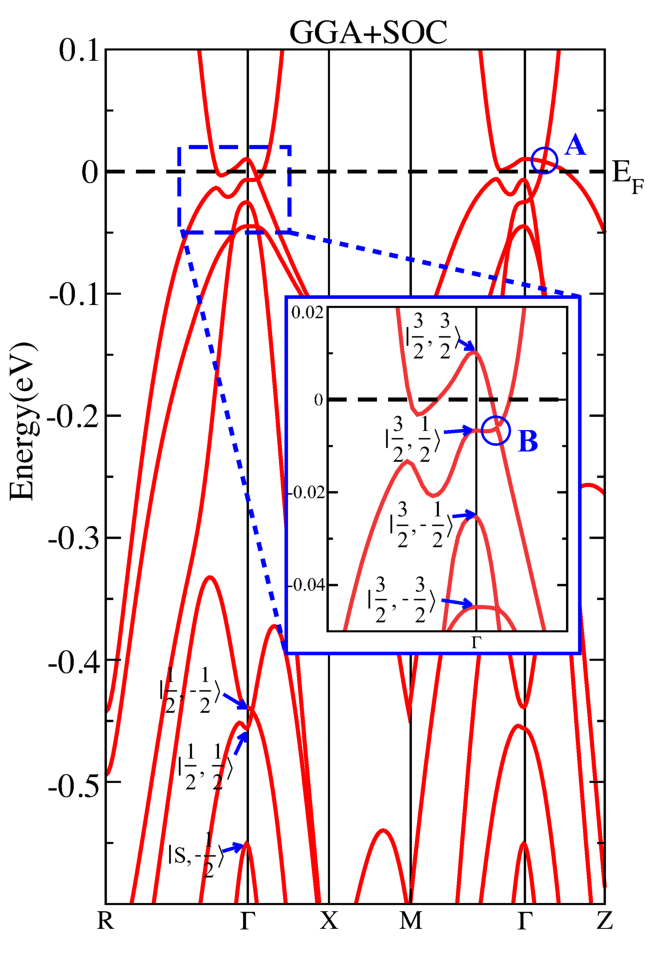
\includegraphics[width=1\linewidth]{bands1.png}
\centering\captionof{figure}{The band structure after including SOC (with majority spin aligning to the
(001) direction), showing two types of crossing, A and B. \cite{xu} \\ \label{bands1}}
\end{minipage}

The founding paper in our case is Xu et al. (2011) \cite{xu}, that was first to present band structure calculation of the material, with spin-orbit coupling (SOC) included using the WIEN2k package with the generalized gradient approximation (GGA). Excluding SOC the material is approximately characterized as a “zero-gap half-metal”, as it is almost a half-metal because of the presence of a gap in the up-spin channel just above the Fermi level; while it is nearly zero-gapped because of the band-touching around the $\Gamma$ point just below Fermi level in the down spin channel (see Fig.~\ref{bands0}). Including SOC they find two kinds of band-crossings near the Fermi level (called A and B in Fig.~\ref{bands1}). The crossing-B is found to be accidental, while the crossing-A are located at the phase boundary between C = 2 and C = 0 planes, and therefore are topologically unavoidable Weyl nodes. This also means that the fermi arcs should be stable as well, making our material a much better Weyl semimetal candidate, then recently discussed pyrochlore iridates.

Guo et al. (2012) \cite{guo} repeated their calculations and also explored the structure with a modified Becke and Johnson exchange potential (mBJLDA), that allowed the study of pressure induced semiconductor-metal transitions. The latter method yielded a more accurate band gap value, however SOC was not included.

The existence of band crossing points was also confirmed using two-band $\bm{k} \cdot \bm{p}$ theories (Fang et al. (2012) \cite{fang}), identifying it to exhibit a double-Weyl semimetal phase. They also propose the splitting of multi-Weyl nodes by applying a symmetry-breaking strain, a potentially fruitful experimental probe.

%%%%%%%%%%%%%%%%%%%%%%%%%%%%%%%%%%%%%%%%%%%%%%%%%%%%%%%%%%%
%%%%%%%%%%%%%%%%%%%%%%%%%%%%%%%%%%%%%%%%%%%%%%%%%%%%%%%%%%%

\section{Specific heat}

The recent interest in HgCr$_2$Se$_4$ also resulted in papers that explore fundamental properties previously not discussed, allowing us a more complete characterization of the material. One of these papers is previously mentioned Wang et al. (2012) \cite{wang}, the core paper on low temperature characterization, mostly detailing the specific heat of the material, but it also contains new insight about its magnetic properties (see Fig.~\ref{dheat} for the divergence of $C_p$). Specific heat was measured on a single crystal between 2 K to 300 K, as shown in Fig.~\ref{heat}. \\


\noindent\begin{minipage}{.44\linewidth}
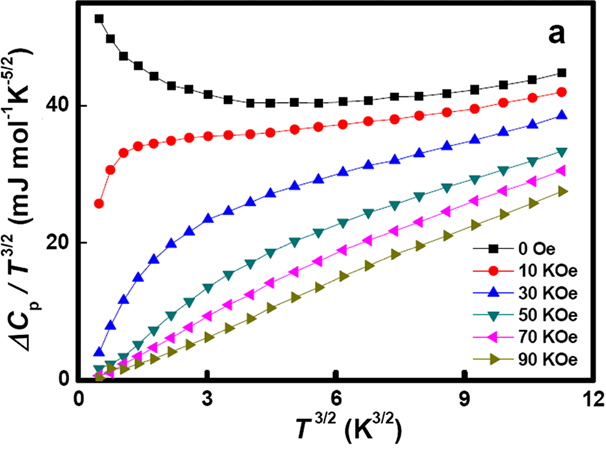
\includegraphics[width=1\linewidth]{dheatvstemp.png}
\centering\captionof{figure}{The divergence from $C_p=\alpha T+\delta T^{3/2}+\beta_DT^3$ at low temperatures indicating the competition between FM and AFM orders \cite{wang}.\label{dheat}}
\end{minipage}%
~ ~ ~ ~
\begin{minipage}{0.54\linewidth}
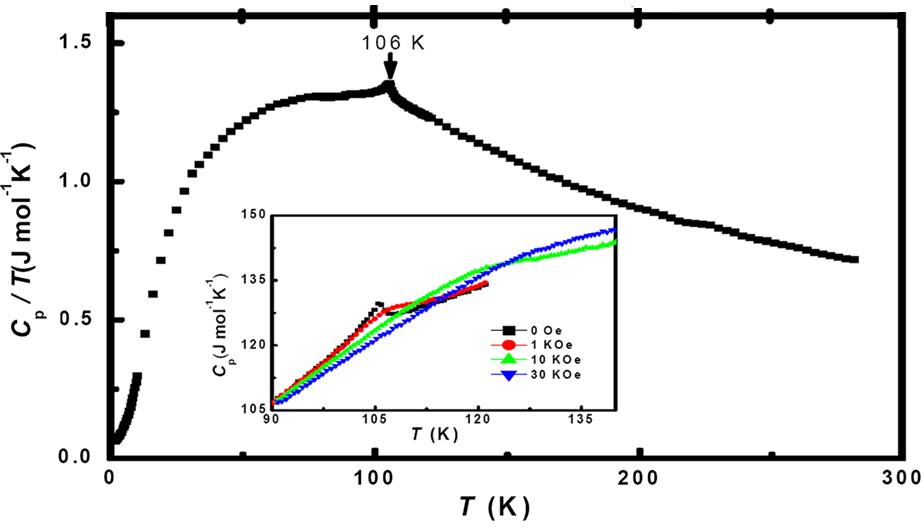
\includegraphics[width=1.07\linewidth]{heatvstemp.png}
\centering\captionof{figure}{The specific heat in the form $C_p$/$T$ vs. $T$. The inset shows the
vicinity of the magnetic transition at 106 K at different magnetic fields \cite{wang}. \label{heat}}
\end{minipage}

%%%%%%%%%%%%%%%%%%%%%%%%%%%%%%%%%%%%%%%%%%%%%%%%%%%%%%%%%%%
%%%%%%%%%%%%%%%%%%%%%%%%%%%%%%%%%%%%%%%%%%%%%%%%%%%%%%%%%%%
 
\section{Conclusions and future work}
\label{sec:conclusion}

%Weyl nodes are stable as long as charge conservation and translational invariance is preserved. Disorder, in general, does not preserve the latter symmetry; however, if the disorder is smooth, many properties of the WSM that rely on the topological nature of the band structure should survive.

%This material has magnetic order, thus time-reversal symmetry is broken, so a Weyl semimetal phase can only be realized with unbroken inversion symmetry.

We have provided a summary of the literature on HgCr$_2$Se$_4$,  spanning five sections. The goal was to uncover previous findings that can be related to future work on experimentally identifying the material's Weyl semimetal nature.

It is important to recap three key features of a Weyl semimetal. These are obvious band intersections, surface states known as Fermi arcs (observable by ARPES), and chiral anomaly. The latter comes with anomalous transport properties (such as negative contribution to magnetoresistance, anomalous Hall effect, slow decay of a voltage in the presence of a magnetic field \cite{hosur}). HgCr$_2$Se$_4$ has to potential to exhibit all of these.


%\begin{acknowledgments}
%\end{acknowledgments}
%%%%%%%%%%%%%%%%%%%%%%%%%%%%%%%%%%%%%%%%%%%%%%%%%%%%%%%%%%%
%%%%%%%%%%%%%%%%%%%%%%%%%%%%%%%%%%%%%%%%%%%%%%%%%%%%%%%%%%%



\bibliography{report}{}
\bibliographystyle{unsrt}

\end{document}             % End of document.

